%%%%%%%%%%%%%%%%%%%%%%%%%%%%%%%%%%%%%%%%%%%%%%%%%%%%%%%%%%%%%%%%%%%%%%
% How to use writeLaTeX: 
%
% You edit the source code here on the left, and the preview on the
% right shows you the result within a few seconds.
%
% Bookmark this page and share the URL with your co-authors. They can
% edit at the same time!
%
% You can upload figures, bibliographies, custom classes and
% styles using the files menu.
%
%%%%%%%%%%%%%%%%%%%%%%%%%%%%%%%%%%%%%%%%%%%%%%%%%%%%%%%%%%%%%%%%%%%%%%



\documentclass[12pt]{article}

\usepackage{sbc-template} 
\usepackage{graphicx,url}

%\usepackage[brazil]{babel}   
\usepackage[utf8]{inputenc}  

     
\sloppy

\title{Vpns e seus usos na computação moderna\\ Artigo e Resumo}

\author{Pedro Henrique Bufulin de Almeida \inst{1}, Gabriel Solis Corrêa\inst{2},\\ Mateus Pereira da Silva\inst{3}, Bruno Falbo Zanotelli\inst{4} }


\address{Faculdade de Computação -- Universidade Federal de Uberlândia (UFU)
  \\Caixa Postal 593 -- CEP 38.400-902 -- Uberlândia -- MG -- Brazil
  \email{pedrohba18@gmail.com, gsolis.comp@gmail.com,}
  \email{mateus1128@gmail.com, brunofalbo@hotmail.com}
}


\begin{document} 

\maketitle
     
\begin{resumo} 
  Presente Artigo visa explorar as VPNs, seus usos na computação moderna
  e ferramentas relacionadas, além de conceituar o termo VPN. Serão realizados
  e documentados testes utilizando a ferramenta OpenVPN em um sistema de máquinas Ubuntu,
  hospedados nos servidores da Digital Ocean, para observar o funcionamento e as
  limitações de uma VPN.
\end{resumo}

\section{O que é uma VPN?}

VPN, Virtual Private Network, ou melhor dizendo em português, Rede Virtual Privada,
vem se tornando cada vez mais comum no mercado tecnológico, encontramos nas lojas de aplicativos e softwares,
vários aplicativos de VPN, mas o que exatamente é uma VPN?
Resumidamente é um túnel seguro criado nada rede de comunicação entre o dispositivo e a Internet,
o que garante a segurança dos dados trafegados nessa rede de comunicação.
Em outra palavras, é codificar os dados que são trocados entre o dispositivo e a internet,
para tornar sua interceptação mais difícil, além de poder fornecer acesso restrito a quem tem as
credenciais necessárias. Extremamente recomendado para utilizar em locais com rede pública, como areoportos e shopping centers,
assim seus dados estariam criptografados, e se um invasor estiver analisando o trafego de dados,
encontrará apenas caracteres sem o menor sentido, porque seus dados de navegação estão todos criptografados,
evitando assim espionagem ("man-in-the-middle"), roubo de dados, ataque de hackers, entre outros.

\center
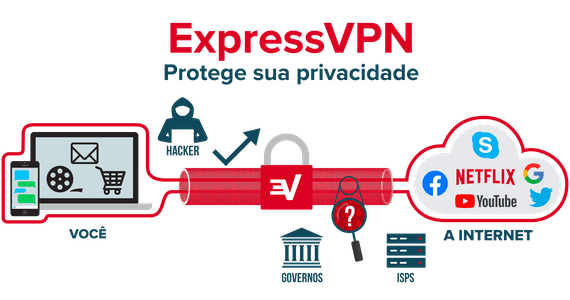
\includegraphics[width=10cm]{images/what-is-vpn-pt_3x.png}

\section{Configurado uma VPN utilizando OpenVPN}

\subsection{Quais os protocolos são utilizados em VPN?}
Protocolos são essenciais na escolha do servidor VPN, já que é um elemento suma importância para esse serviço.

Os protocolos são a combinação de padrões de criptografia e de transmissão, que concedem rápido acesso e segurança aos servidores VPN.

Existem vários tipos, dentre eles:

\subsubsection{PPTP}
Como uma extensão do Point-to-Point Protocol (PPP), o PPTP (Point-to-Point Tunneling Protocol) é um protocolo de servidor VPN muito utilizado e suportado pelos dispositivos. Ele possui uma criptografia mais básica, o que pode deixar a desejar na questão de segurança dos dados. 

Contudo, essa característica também faz com que ele seja mais rápido do que outros modelos de protocolo VPN, além de possuir configuração mais simples. A maior parte das falhas de segurança também já foram resolvidas nas versões mais atuais do PPTP. Isso faz com que essa maior agilidade compense em detrimento de uma menor segurança para algumas empresas.

Uma forma de melhorar a segurança é utilizar da tecnologia PPP ou Protocolo Ponto-a-Ponto para implementar medidas de criptografia.

Esta é uma VPN útil tanto para os usuários empresariais, como, para usuários domésticos. São ideais para uso pessoal e empresarial, porque elas não exigem a compra e a instalação de hardware e recursos extras, normalmente oferecidos como software add-on barato. Além de serem compatíveis com os sistemas Linux, Windows e Mac.

\subsubsection{L2TP}
O L2TP (Layer 2 Tunneling Protocol) consegue garantir confidencialidade, autenticação e integridade de dados, o que assegura maior proteção. No entanto, nada disso é oferecido pelo protocolo por si só. Pois ele se baseia em um protocolo de criptografia IPSec para proporcionar a privacidade necessária aos usuários da rede.

As ligações do L2TP são conhecidas como linhas virtuais e oferecem mais facilidades para aqueles que utilizam o servidor de forma remota. Isso porque ele possibilita que o servidor da rede VPN de uma organização consiga gerir os endereços IP atribuídos aos seus usuários. Assim, garantindo proteção e privacidade.

\subsubsection{IPSec}
IPSec (Internet Protocol Security) oferece transferência estável de dados pela rede pública ou privada. Uma extensão do protocolo IP (Internet Protocol), ele visa garantir mais segurança na comunicação, utilizando-se de serviços de segurança criptográficos. 

Sua forma de funcionamento se dá da seguinte maneira: é necessário pegar um pacote IP privado, criptografar, autenticar e dar integridade e depois encapsular os pacotes protegidos para novos IPs a serem repassados.

Com esta maneira operacional, o IPSec se torna um bom protocolo em segurança para as empresas, filiais e usuários remotos. Dentre as suas principais vantagens e benefícios, podemos destacar também o oferecimento de um alto nível de confidencialidade, privacidade e autenticação dos dados e informações que trafegam dentro da rede.


\subsection{Pontos fortes e fracos de uma VPN}

O uso de um servidor VPN é principalmente recomendado para empresas. Pois consegue manter informações seguras nas comunicações remotas ou em armazenamento em nuvem.

Servidores com tal configuração, trazem algumas vantagens para os usuários, como:

\subsubsection{Segurança}

Principal ponto positivo do servidor VPN.  Por usar criptografia dos dados e diversos outros recursos de segurança, ele permite que a navegação seja mais confiável e segura, independente de onde seja usada e em qual rede acessada.

\subsubsection{Privacidade}
As informações que estão na rede só são acessadas por quem tem permissão. Assim, cada indivíduo tem acesso apenas ao que é de seu interesse para o trabalho e nada mais. Dessa forma, todas as informações e dados que circulam dentro da rede da empresa acabam sendo mais confiáveis e úteis. 

A privacidade dos usuários que utilizam a rede com servidor VPN estará garantida, sem riscos de que informações confidenciais sejam vazadas.

\subsubsection{Acesso remoto}
Desde que, aqueles com permissão tenham acesso a internet, será garantido acessar os servidores remotos, não importando o lugar do mundo ou o dispositivo. 

Tal característica permite que, funcionários trabalhem remotamente sem que precisem carregar notebooks da empresa ou anotem informações importantes quando tiverem a distância. Tornando o trabalho mais simples e tendo um ganho considerável em produtividade.

A empresa também se beneficia pois, deixa de ser necessário investir em equipamentos e tecnologias que garantiriam o acesso e segurança aos sistemas. Assim como funcionários podem passar a usar seus próprios dispositivos.

\subsubsection{Custo}
Servidores VPN são consideravelmente mais baratos do que outras tecnologias e configurações de segurança.

Como utilizam a rede pública de internet como conexão, diminui-se os custos de implantação e softwares próprios.


Porém, todo e qualquer sistema ou tecnologia apresentam desvantagens, no caso de servidores VPN, essas são as principais:

\subsubsection{Velocidade}
Principal ponto negativo de servidores VPN. Para utilizar esse tipo de servidor é preciso estabelecer duas conexões.

Logo, uma boa velocidade de rede é exigida, e mesmo assim, é quase sempre bem perceptível a queda na banda de internet utilizada.

\subsubsection{Dependência da Internet}
O acesso remoto é algo extremamente útil para se trabalhar fora da empresa porém, um acesso constante a internet é necessário.

Se a rede tem uma conexão instável, cai frequentemente ou se não possui acesso a internet, não será possível acessar o servidor VPN e os dados nele armazenados.

\subsubsection{Confiança no Servidor}
Existem muitos serviços de VPN sendo oferecidos, alguns gratuitos, a preços baixos ou outros que necessitam de um investimento maior.

Com tanta oferta, é importante entender as necessidades da sua rede, antes de contratar algum serviço.  As VPNs constantemente mudam. Por isso, é importante ter um suporte em que a empresa consiga facilmente entrar em contato para resolver os impasses da rede.

Uma outra opção, seria a empresa criar a sua própria rede de servidores VPN, utilizando tecnologias Open Source, tais como, a OpenVPN. Tópico esse, que será abordado mais a frente.


\subsection{Configurado uma VPN utilizando OpenVPN}

Para que seja possível implementar uma VPN como neste exemplo, você precisará
de uma máquina rodando Ubuntu versão 18.04. Por questões de praticidade, não será
visto com profundidade todo o processo de instalação das ferramentas que serão usadas, sendo algumas 
apenas mencionadas cabendo ao leitor descobrir como instalá-las. Além do servidor mencionado,
o ideal seria ter uma outra máquina para ser a autoridade de certificação (CA), para evitar
que um agressor capaz de se infiltrar no servidor consiga acessar a chave privada
e assinar novos certificados. 

\subsection{Instalando os programas necessários}

O primeiro passo é instalar o \emph{OpenVPN} que está disponível nos repositórios padrão do ubuntu.
Em seguida, instale \emph{EasyRCA} tanto na máquina CA quanto no servidor que servira o VPN.
O repositório deste programa encontra-se no github no mesmo repositório do \emph{OpenVPN}. 
A versão a ser utilizada é a 3.0.8.

\subsection{Configurando as variáveis e construindo o CA}

No máquina que contém o CA, entre no diretório onde foi extraído o \emph{EasyRCA}. copie o conteúdo
do arquivo \texttt{vars.example} para um outro arquivo onde serão armazenadas as variáveis. Atualize
os valores de acordo com suas informações, feche e salve o arquivo. 

Dentro do da mesma pasta, existe um\emph{script} chamado \texttt{easyrca}. Execute-o da seguinte
maneira: \texttt{./easyrsa init-pki}. Isso irá iniciar a infraestrutura de chaves públicas no servidor CA.
Se der tudo certo, deve surgir um diretório chamado \texttt{pki}. Em seguida, chame o script anterior 
novamente mas dessa vez com a opção \texttt{build-ca}. Isso irá construir a CA e criar
dois arquivos importantes. Um deles é um certificado público que no contexto de uma VPN para informar
ao servidor e ao cliente que ambos fazem parte da mesma rede. Isso serve como defesa de ataques 
do tipo \emph{man-in-the-middle} 



\section{Discussão}

% Section titles must be in boldface, 13pt, flush left. There should be an extra
% 12 pt of space before each title. Section numbering is optional. The first
% paragraph of each section should not be indented, while the first lines of
% subsequent paragraphs should be indented by 1.27 cm.

\section{Considerações Finais}


% Figure and table captions should be centered if less than one line
% (Figure~\ref{fig:exampleFig1}), otherwise justified and indented by 0.8cm on
% both margins, as shown in Figure~\ref{fig:exampleFig2}. The caption font must
% be Helvetica, 10 point, boldface, with 6 points of space before and after each
% caption.

% \begin{figure}[ht]
% \centering
% 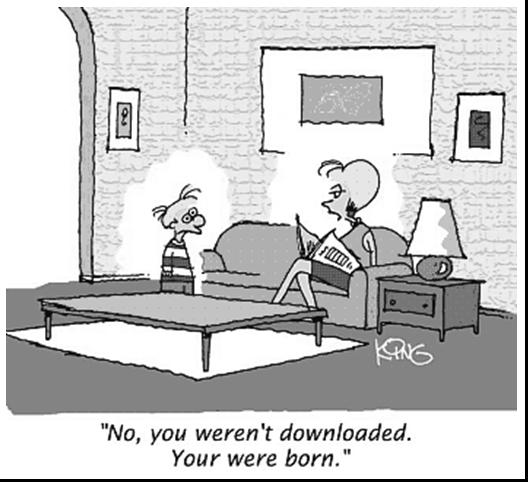
\includegraphics[width=.5\textwidth]{fig1.jpg}
% \caption{A typical figure}
% \label{fig:exampleFig1}
% \end{figure}

% \begin{figure}[ht]
% \centering
% 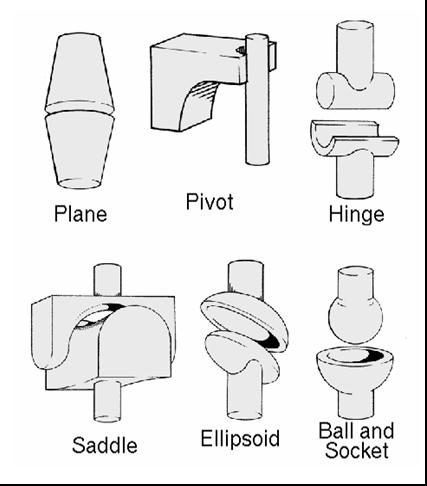
\includegraphics[width=.3\textwidth]{fig2.jpg}
% \caption{This figure is an example of a figure caption taking more than one
%   line and justified considering margins mentioned in Section~\ref{sec:figs}.}
% \label{fig:exampleFig2}
% \end{figure}

% In tables, try to avoid the use of colored or shaded backgrounds, and avoid
% thick, doubled, or unnecessary framing lines. When reporting empirical data,
% do not use more decimal digits than warranted by their precision and
% reproducibility. Table caption must be placed before the table (see Table 1)
% and the font used must also be Helvetica, 10 point, boldface, with 6 points of
% space before and after each caption.

% \begin{table}[ht]
% \centering
% \caption{Variables to be considered on the evaluation of interaction
%   techniques}
% \label{tab:exTable1}
% 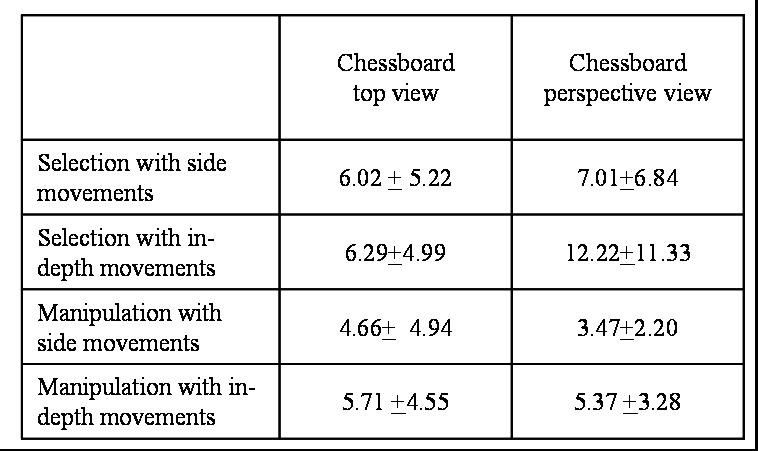
\includegraphics[width=.7\textwidth]{table.jpg}
% \end{table}

\section{Referências}

Bibliographic references must be unambiguous and uniform.  We recommend giving
the author names references in brackets, e.g. \cite{knuth:84},
\cite{boulic:91}, and \cite{smith:99}.

The references must be listed using 12 point font size, with 6 points of space
before each reference. The first line of each reference should not be
indented, while the subsequent should be indented by 0.5 cm.

\bibliographystyle{sbc}
\bibliography{sbc-template}

\end{document}
